\section{Einphasige Brückenschaltung - Ungesteuerter Betrieb}

\subsection{Messschaltung}

\begin{figure}[h!]
    \centering
    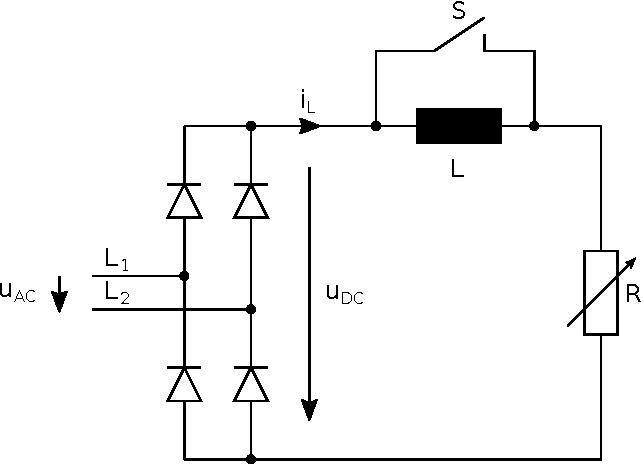
\includegraphics[scale=\sscale]{./../fig/b2_diode.pdf}
    \caption{B2 Diodengleichichter}
\end{figure}

\subsection{Messungen}

\begin{figure}[h!]
    \centering
    \includegraphics[scale=\pscale]{./../plots/631_01.pdf}
    \caption{B2 Diodengleichrichter mit L-Glättung, Lastposition 16}
\end{figure}

\begin{figure}[h!]
    \centering
    \includegraphics[scale=\pscale]{./../plots/631_02.pdf}
    \caption{B2 Diodengleichrichter mit L-Glättung, Lastposition 11}
\end{figure}

\begin{figure}[h!]
    \centering
    \includegraphics[scale=\pscale]{./../plots/631_03.pdf}
    \caption{B2 Diodengleichrichter mit L-Glättung, Lastposition 6}
\end{figure}

\begin{figure}[h!]
    \centering
    \includegraphics[scale=\pscale]{./../plots/631_04.pdf}
    \caption{B2 Diodengleichrichter ohne Glättung, Lastposition 16}
\end{figure}

\begin{figure}[h!]
    \centering
    \includegraphics[scale=\pscale]{./../plots/631_05.pdf}
    \caption{B2 Diodengleichrichter ohne Glättung, Lastposition 11}
\end{figure}

\begin{figure}[h!]
    \centering
    \includegraphics[scale=\pscale]{./../plots/631_06.pdf}
    \caption{B2 Diodengleichrichter ohne Glättung, Lastposition 6}
\end{figure}


\clearpage
